\documentclass[11pt, oneside]{article}    % use "amsart" instead of "article" for AMSLaTeX format
\usepackage{geometry}                   % See geometry.pdf to learn the layout options. There are lots.
\geometry{letterpaper}                      % ... or a4paper or a5paper or ... 
%\geometry{landscape}                   % Activate for for rotated page geometry
\usepackage[parfill]{parskip}       % Activate to begin paragraphs with an empty line rather than an indent
\usepackage{graphicx}       % Use pdf, png, jpg, or eps§ with pdflatex; use eps in DVI mode
                % TeX will automatically convert eps --> pdf in pdflatex  
                
\setlength{\topmargin}{-0.5in}
\setlength{\textheight}{9in}
\setlength{\textwidth}{7in}
\setlength{\oddsidemargin}{-.25in}

\title{Assignment 5: K-Means Clustering}
\author{Ryan Bernstein}
%\date{}

\begin{document}
\maketitle

\section{Experiment 1}

This experiment does deviate slightly from the assignment specification. With random cluster centers, accuracy wasn't great, and the visualizations were difficult to decipher.

To address this, I abandoned the random initial centering in favor of an algorithm described in the reading. Namely, we start with one random initial cluster center, then center successive clusters on the data points (in the training set) that are furthest from any preexisting cluster center.

There is still an element of randomness to this, to be sure, but its effect should be greatly reduced. I abandoned the five random restarts after making this change due to how long the 30-cluster experiment was taking (due to the additional computations required for this new, non-random strategy).

If you'd like to see results for the random-restart strategy detailed in the assignment spec, my implementation is still capable of doing this. Simply uncomment the calls to \texttt{ClusterSet.bestOf()} in \texttt{main.swift} (and comment the alternate initializations where appropriate).

Other than that, this is a pretty standard K-Means clustering algorithm. We repeat the following steps until either cluster centers stop moving or until we hit some arbitrary bound that indicates that we may be oscillating. This bound was 1000 iterations, but I don't believe any test run came anywhere close. But back to the steps:
\begin{itemize}
	\item Bucket the instances in the training set to the cluster centers to which they are closest
	\item Move cluster centers to the mean of the instance vectors that have been associated with it
\end{itemize}

Once this is done, we can bucket our training instances one final time and associate a guess with each cluster based on the values that appear most often. We can then bucket test instances and assign the cluster guesses to them as a means of classification.

\begin{verbatim}
Training SSE: 2859972.98448893
Training SSS: 65745.6972561082
Mean entropy: 1.49867133967332
Accuracy: 0.613800779076238
\end{verbatim}

\begin{center}
	\begin{tabular}{|c|c|c|c|c|c|c|c|c|c|c|}
		\hline
		& \textbf{0} & \textbf{1} & \textbf{2} & \textbf{3} & \textbf{4} & \textbf{5} & \textbf{6} & \textbf{7} & \textbf{8} & \textbf{9} \\ \hline
		\textbf{0} & 135 & 0 & 0 & 26 & 5 & 8 & 4 & 0 & 0 & 0 \\ \hline
		\textbf{1} & 0 & 57 & 26 & 0 & 0 & 1 & 3 & 0 & 95 & 0 \\ \hline
		\textbf{2} & 2 & 2 & 149 & 12 & 0 & 0 & 0 & 2 & 10 & 0 \\ \hline
		\textbf{3} & 55 & 0 & 9 & 100 & 0 & 2 & 0 & 5 & 12 & 0 \\ \hline
		\textbf{4} & 0 & 5 & 0 & 0 & 150 & 2 & 0 & 8 & 16 & 0 \\ \hline
		\textbf{5} & 37 & 1 & 0 & 25 & 1 & 117 & 1 & 0 & 0 & 0 \\ \hline
		\textbf{6} & 2 & 1 & 0 & 0 & 1 & 1 & 176 & 0 & 0 & 0 \\ \hline
		\textbf{7} & 0 & 0 & 0 & 0 & 0 & 0 & 0 & 111 & 68 & 0 \\ \hline
		\textbf{8} & 36 & 8 & 4 & 8 & 0 & 7 & 1 & 2 & 108 & 0 \\ \hline
		\textbf{9} & 88 & 17 & 2 & 57 & 0 & 3 & 0 & 12 & 1 & 0 \\ \hline
	\end{tabular}
\end{center}

Interestingly, we don't seem to have labeled any instances as 9. This is probably to be expected. Since we have ten different digits and ten different clusters, any digit that appears in more than one cluster means that some other digit can't be identified.

Let's look now at the visualizations that resulted from these cluster centers:
\begin{center}
	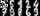
\includegraphics{Exp1Visualizations}
\end{center}

With the exception of the first cluster, everything is a (mostly) recognizable digit. This was not the case with random initial cluster centers, which is ultimately why I decided to deviate from the assignment spec.

The first cluster center is still randomly assigned, and I'm assuming that this is the reason for the strangeness of its visualization. I had assumed that this would sort itself during the recentering process, but perhaps not.

\section{Experiment 2}

This is the same as last time, but now we have 30 cluster centers instead of 10. As expected (or at least, as I expected), accuracy is higher than last time:

\begin{verbatim}
Experiment 2
Training SSE: 2092880.32205385
Training SSS: 700548.594357255
Mean entropy: 0.765311164908606
Accuracy: 0.781302170283806
Program ended with exit code: 0
\end{verbatim}

I attribute this to the fact that with extra cluster centers, we're able to have separate clusters for things like open/closed fours or sevens with/without crosses. This should hopefully reduce ambiguity for ``sub-clusters'' that --- if we only had one cluster per digit --- would appear to be between digits.

\begin{center}
	\begin{tabular}{|c|c|c|c|c|c|c|c|c|c|c|}
		\hline
		& \textbf{0} & \textbf{1} & \textbf{2} & \textbf{3} & \textbf{4} & \textbf{5} & \textbf{6} & \textbf{7} & \textbf{8} & \textbf{9} \\ \hline
		\textbf{0} & 175 & 0 & 0 & 0 & 3 & 0 & 0 & 0 & 0 & 0 \\ \hline
		\textbf{1} & 0 & 124 & 50 & 0 & 0 & 2 & 0 & 0 & 5 & 1 \\ \hline
		\textbf{2} & 0 & 10 & 159 & 0 & 0 & 0 & 5 & 2 & 1 & 0 \\ \hline
		\textbf{3} & 1 & 0 & 6 & 135 & 0 & 4 & 0 & 7 & 4 & 26 \\ \hline
		\textbf{4} & 0 & 6 & 0 & 0 & 153 & 1 & 0 & 0 & 10 & 11 \\ \hline
		\textbf{5} & 1 & 0 & 0 & 11 & 1 & 154 & 0 & 0 & 0 & 15 \\ \hline
		\textbf{6} & 1 & 4 & 0 & 0 & 1 & 13 & 162 & 0 & 0 & 0 \\ \hline
		\textbf{7} & 0 & 0 & 1 & 0 & 1 & 0 & 0 & 174 & 0 & 3 \\ \hline
		\textbf{8} & 0 & 16 & 23 & 6 & 0 & 17 & 0 & 1 & 107 & 4 \\ \hline
		\textbf{9} & 0 & 4 & 1 & 96 & 9 & 7 & 0 & 0 & 2 & 61 \\ \hline
	\end{tabular}
\end{center}

We do seem to have resolved our issues with classifying nines, although this is still the digit for which we have the lowest correctness. We've identified many nines as threes, and conversely, many threes as nines. We also saw relatively high numbers of fours and fives classified as nines.

\begin{center}
	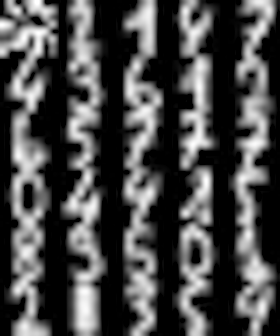
\includegraphics{Exp2Visualizations}
\end{center}

Most of these are actually decently recognizable, although there are a couple of mysteries (notably, the first example and the one in the second-to-last column third from the bottom). I interpret the fact that the first cluster is again undecipherable as evidence for my hypothesis regarding the random initial cluster center.

\section{Running this Code}

As this implementation is written in Swift, it can only be run on OS X.

I would recommend creating a new Swift project in Xcode and importing all of the Swift files. Alternately, you could copy/paste each of the class files into the Swift REPL, but this would be considerably more work.

This program also expects some command-line input. If you are running this code in Xcode, you can configure command-line arguments via Project $\rightarrow$ Scheme $\rightarrow$ Edit Scheme. I also configured \texttt{main.swift} to prompt the user for input if no arguments were given.

Specifically, the arguments expected are:
\begin{enumerate}
	\item The location of the training data file
	\item The location of the test data file
	\item The directory where output (cluster visualizations and confusion matrices) should be written.
\end{enumerate}

If you're having trouble getting the code to run, please do let me know and I'd be happy to assist.

\end{document}